\documentclass[border=5pt]{standalone}
\usepackage[T1]{fontenc}
\RequirePackage[semibold]{sourcesanspro}
\usepackage{pgfplots}
\usepackage{xcolor}

\pgfplotsset{compat=1.18}

% Define colors
\definecolor{nonebar}{HTML}{333333}
\definecolor{drybar}{HTML}{C62828}
\definecolor{npxxybar}{HTML}{00897B}
\definecolor{cwxpbar}{HTML}{FF9800}
\definecolor{pifbar}{HTML}{9E9E9E}
\definecolor{textgray}{HTML}{404040}
\definecolor{gridgray}{HTML}{E0E0E0}

\begin{document}
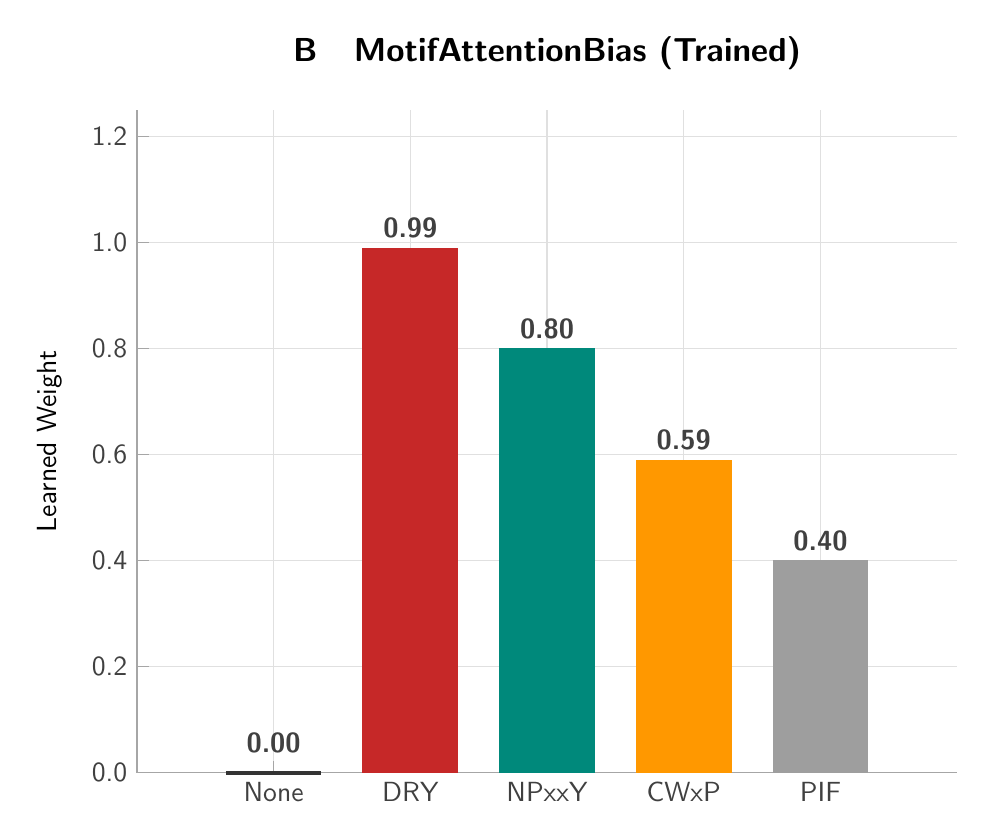
\begin{tikzpicture}

\begin{axis}[
    font=\footnotesize\sffamily,
    width=12cm,
    height=10cm,
    ymin=0,
    ymax=1.25,
    xmin=0,
    xmax=6,
    xtick={1,2,3,4,5},
    xticklabels={None, DRY, NPxxY, CWxP, PIF},
    xticklabel style={font=\normalsize\sffamily, color=textgray},
    ytick={0.0, 0.2, 0.4, 0.6, 0.8, 1.0, 1.2},
    yticklabels=\empty,
    yticklabel style={font=\normalsize\sffamily, color=textgray},
    ylabel={Learned Weight},
    ylabel style={font=\normalsize\sffamily, at={(-0.08,0.5)}},
    title={\textbf{B\quad MotifAttentionBias (Trained)}},
    title style={font=\large\sffamily\bfseries, at={(0.5,1.02)}},
    axis line style={gray!70, line width=0.5pt},
    tick style={gray!70},
    ymajorgrids=true,
    xmajorgrids=true,
    grid style={gridgray, line width=0.5pt},
    axis x line*=bottom,
    axis y line*=left,
    clip=false,
]

% Manually draw y-axis labels (no loops)
\node[font=\normalsize\sffamily, color=textgray, anchor=east] at (axis cs:0,0.0) {0.0};
\node[font=\normalsize\sffamily, color=textgray, anchor=east] at (axis cs:0,0.2) {0.2};
\node[font=\normalsize\sffamily, color=textgray, anchor=east] at (axis cs:0,0.4) {0.4};
\node[font=\normalsize\sffamily, color=textgray, anchor=east] at (axis cs:0,0.6) {0.6};
\node[font=\normalsize\sffamily, color=textgray, anchor=east] at (axis cs:0,0.8) {0.8};
\node[font=\normalsize\sffamily, color=textgray, anchor=east] at (axis cs:0,1.0) {1.0};
\node[font=\normalsize\sffamily, color=textgray, anchor=east] at (axis cs:0,1.2) {1.2};

% Bar width in axis units
\pgfmathsetmacro{\barwidth}{0.35}

% None bar (height 0, just a line)
\fill[nonebar] (axis cs:1-\barwidth,0) rectangle (axis cs:1+\barwidth,0.001);
\draw[nonebar, line width=1.5pt] (axis cs:1-\barwidth,0) -- (axis cs:1+\barwidth,0);
\node[font=\normalsize\sffamily\bfseries, color=textgray, above] at (axis cs:1,0.02) {0.00};

% DRY bar
\fill[drybar] (axis cs:2-\barwidth,0) rectangle (axis cs:2+\barwidth,0.99);
\node[font=\normalsize\sffamily\bfseries, color=textgray, above] at (axis cs:2,0.99) {0.99};

% NPxxY bar
\fill[npxxybar] (axis cs:3-\barwidth,0) rectangle (axis cs:3+\barwidth,0.80);
\node[font=\normalsize\sffamily\bfseries, color=textgray, above] at (axis cs:3,0.80) {0.80};

% CWxP bar
\fill[cwxpbar] (axis cs:4-\barwidth,0) rectangle (axis cs:4+\barwidth,0.59);
\node[font=\normalsize\sffamily\bfseries, color=textgray, above] at (axis cs:4,0.59) {0.59};

% PIF bar
\fill[pifbar] (axis cs:5-\barwidth,0) rectangle (axis cs:5+\barwidth,0.40);
\node[font=\normalsize\sffamily\bfseries, color=textgray, above] at (axis cs:5,0.40) {0.40};


\end{axis}

\end{tikzpicture}
\end{document}